% Dit werk is gelicenseerd onder de licentie Creative Commons Naamsvermelding-GelijkDelen 4.0 Internationaal. Ga naar http://creativecommons.org/licenses/by-sa/4.0/ om een kopie van de licentie te kunnen lezen.
\documentclass[t]{beamer}

% vaak gebruikte packages, nederlands
\usepackage[margin=2.5cm]{geometry}     % Marges instellen
\usepackage[dutch]{babel}               % Voor nederlandstalige hyphenatie (woordsplitsing)
\usepackage{amsmath,amsthm}             % Uitgebreide wiskundige mogelijkheden
\usepackage{url}                        % Om url's te verwerken
\usepackage{graphicx,subfigure}         % Om figuren te kunnen verwerken
\usepackage{color}
\usepackage{framed}
\usepackage{multicol}
\usepackage[small,bf,hang]{caption}     % Om de captions wat te verbeteren
\usepackage[utf8]{inputenc}             % Om niet ascii karakters rechtstreeks te kunnen typen
\usepackage{float}                      % Om nieuwe float environments aan te maken. Ook optie H!
\usepackage{flafter}                    % Opdat floats niet zouden voorsteken
\usepackage[section]{placeins}			% Om ervoor te zorgen dat floats binnen dezelfde section blijven
\usepackage[nottoc]{tocbibind}			% Bibliografie en inhoudsopgave in ToC; zie tocbibind.dvi
\usepackage{fancyhdr}                   % Voor fancy headers en footers
\usepackage{thmtools}                   % theorem tools
\usepackage{parskip}                    % Om paragrafen met een verticale spatie ipv horizontaal te laten beginnen
\usepackage[plainpages=false]{hyperref} % Om hyperlinks te hebben in het pdfdocument.



%%%%%%%%%%%%%%%%%%%%%%%%%%%%%%
% Algemene instellingen van het document.
%%%%%%%%%%%%%%%%%%%%%%%%%%%%%%
\renewcommand{\baselinestretch}{1.2} 	% De interlinie afstand wat vergroten.
\setcounter{MaxMatrixCols}{50}          % Max 20 kolommen in een matrix


%%%%%%%%%%%%%%%%%%%%%%%%%%%%%%
% Headers en footers
%%%%%%%%%%%%%%%%%%%%%%%%%%%%%%
\pagestyle{fancy}
\fancyhf{}
\renewcommand{\headrulewidth}{0pt}
\fancyhead[RO] {\rightmark}
\fancyhead[LE] {\leftmark}
\fancyfoot[RO,LE] {\thepage}

% no dot after chapter number
\renewcommand{\chaptermark}[1]{
	\markboth{\MakeUppercase{ \chaptername\ \thechapter\quad #1}}{}
}
% no dot after section number
\renewcommand{\sectionmark}[1]{
	\markright{\MakeUppercase{ \thesection\quad #1}}{}
}

% page header and footer style in mainmatter aanpassen
\let\newmainmatter\mainmatter
\renewcommand{\mainmatter}{

	\pagestyle{fancy}
	\fancyhf{}
	\renewcommand{\headrulewidth}{0pt}
	\fancyhead[RO] {\rightmark}
	\fancyhead[LE] {\leftmark}
	\fancyfoot[RO,LE] {\thepage}
	\fancyfoot[C]{\tiny{Brecht Baeten}}

	\newmainmatter
}
\let\newappendix\appendix
\renewcommand{\appendix}{
	\fancyfoot{}
	\fancyfoot[RO,LE] {\thepage}
	\newappendix
}


%%%%%%%%%%%%%%%%%%%%%%%%%%%%%%
% Nieuwe omgevingen
%%%%%%%%%%%%%%%%%%%%%%%%%%%%%%
\definecolor{shadecolor}{gray}{0.95}
\newcounter{voorbeeldcounter}[chapter]
\renewcommand{\thevoorbeeldcounter}{\thechapter.\arabic{voorbeeldcounter}}
\makeatletter
\newenvironment{voorbeeld}
{
\vspace{3mm}
\addtolength{\leftskip}{5mm}
\begin{shaded*}
\vspace{-3mm}
\refstepcounter{voorbeeldcounter}
\noindent
\textbf{Voorbeeld \thevoorbeeldcounter:\\}
%\vspace{-8mm}
%\begin{multicols}{2}
}
{
%\end{multicols}
\end{shaded*}
\addtolength{\leftskip}{-5mm}
}
\makeatother  
    
%%%%%%%%%%%%%%%%%%%%%%%%%%%%%%
% .svg commando's
%%%%%%%%%%%%%%%%%%%%%%%%%%%%%%
% nieuw commando om svg files dynamisch te updaten
%\newcommand{\executeiffilenewer}[3]{%
%\ifnum\pdfstrcmp{\pdffilemoddate{#1}}%
%{\pdffilemoddate{#2}}>0%
%{\immediate\write18{#3}}\fi%
%}
%% nieuw commando om. svg figuren in te voegen
%% Gebruik: \includesvg{path/filename.svg}
%\newcommand{\includesvg}[2][0]{%
%\executeiffilenewer{#2.svg}{#2.pdf}%
%{inkscape -z -C --file=#2.svg %
%--export-pdf=#2.pdf --export-latex}%
%\ifx#10
%	\let\svgwidth\undefined
%\else
%	\def\svgwidth{#1}
%\fi%
%\input{#2.pdf_tex}%
%\ifx \svgwidth\undefined
%\else
%	\let\svgwidth\undefined
%\fi%
%}

% nieuw commando om .fig figuren in te voegen
\newcommand{\includefig}[2][0]{%
\ifx#10
	\let\figwidth\undefined
\else
	\def\figwidth{#1}
\fi%
\input{#2.pdf_tex}%
\ifx \figwidth\undefined
\else
	\let\figwidth\undefined
\fi%
}

%%%%%%%%%%%%%%%%%%%%%%%%%%%%%%
% Packages
%%%%%%%%%%%%%%%%%%%%%%%%%%%%%%

%\usepackage{geometry}              	% 
\usepackage[dutch]{babel}               % Voor nederlandstalige hyphenatie (woordsplitsing)
\uselanguage{dutch}
\languagepath{dutch}
\usepackage{amsmath,amsthm}             % Uitgebreide wiskundige mogelijkheden
\usepackage{url}                        % Om url's te verwerken
\usepackage{graphicx,subfigure}         % Om figuren te kunnen verwerken
\usepackage[utf8]{inputenc}             % Om niet ascii karakters rechtstreeks te kunnen typen
\usepackage[section]{placeins}			% Om ervoor te zorgen dat floats binnen dezelfde section blijven
\usepackage{multicol}
\usepackage[absolute,overlay]{textpos}

%%%%%%%%%%%%%%%%%%%%%%%%%%%%%%
% Layout
%%%%%%%%%%%%%%%%%%%%%%%%%%%%%%
\usetheme{Frankfurt}
\usefonttheme[onlymath]{serif}
\AtBeginSection[]
{
  \begin{frame}
    \frametitle{Inhoud}
    \tableofcontents[currentsection]
  \end{frame}
}

\setbeamertemplate{navigation symbols}{}
\setbeamertemplate{footline}[page number]

%%%%%%%%%%%%%%%%%%%%%%%%%%%%%%
% Title
%%%%%%%%%%%%%%%%%%%%%%%%%%%%%%
\title{Fluïdummechanica}
\author{Brecht Baeten\inst{1}}
\institute{
	\inst{1}%
  		KU Leuven, Technologie campus Diepenbeek,\\ e-mail: brecht.baeten@kuleuven.be
}
\date{\today}
%%%%%%%%%%%%%%%%%%%%%%%%%%%%%%
% Omgevingen
%%%%%%%%%%%%%%%%%%%%%%%%%%%%%%


\subtitle{Stroming in leidingen}

\begin{document}

	\frame{\titlepage}
%%%%%%%%%%%%%%%%%%%%%%%%%%%%%%%%%%%%%%%%%%%%%%%%%%%%%%%%%%%%%%%%%%%%%%%%%%%
	\section{Inleiding}
	\begin{frame}
		\frametitle{Voorbeeld}
		\center
    	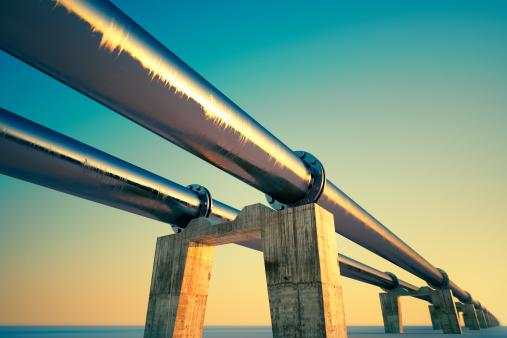
\includegraphics[width=\textwidth]{fig/stroming_in_leidingen/Richard-Steinberg-The-Pipeline-Blog-51.jpg}\\
    	\footnotesize{Bron: http://www.etftrends.com/}
  	\end{frame}
  	\begin{frame}
  		\frametitle{Ontwikkelende stroming}
  		\center
  		\vspace{1.5cm}
  		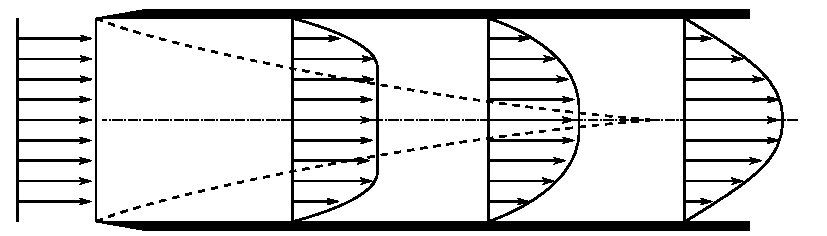
\includegraphics[width=\textwidth]{fig/inwendige_stroming/Ontwikkelende_stroming}
  	\end{frame}	
%%%%%%%%%%%%%%%%%%%%%%%%%%%%%%%%%%%%%%%%%%%%%%%%%%%%%%%%%%%%%%%%%%%%%%%%%%%
  	\section{Dimensieanalyse}
  	\begin{frame}
		\frametitle{Dimensieanalyse}
		\begin{equation*}
			\Delta p = \phi(L,D,v,\mu,\rho)
		\end{equation*}
		\pause
		
		Buckingham Pi, ($n=5$,$k=3$)
		
		\pause
		\begin{equation*}
			\frac{\Delta p}{\frac{1}{2}\rho v^2} = f(L/D,Re)
		\end{equation*}
		\pause
		\begin{equation*}
			\frac{\Delta p}{\frac{1}{2}\rho v^2} = f(Re) \frac{L}{D}
		\end{equation*}
		\pause
		
		\begin{equation}
			\Delta p = f(Re) \frac{1}{2}\rho v^2 \frac{L}{D}
		\end{equation}
	\end{frame}
%%%%%%%%%%%%%%%%%%%%%%%%%%%%%%%%%%%%%%%%%%%%%%%%%%%%%%%%%%%%%%%%%%%%%%%%%%%
  	\section{Laminaire stroming}
  	\begin{frame}
		\frametitle{Snelheidsprofiel}
		\only<1>{
			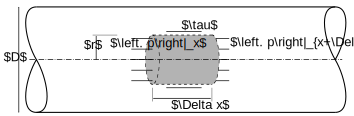
\includegraphics[width=\textwidth]{fig/inwendige_stroming/Laminaire_stroming_in_buis}
		}
		\only<2-9>{
			\begin{textblock}{5}(0,3)
            	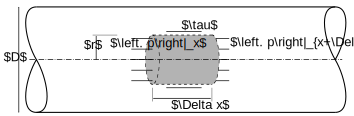
\includegraphics[width=5cm]{fig/inwendige_stroming/Laminaire_stroming_in_buis}
       		\end{textblock}
       		\vspace{2cm}
		}
		\only<2-5>{
			Behoud van impuls in de stromingsrichting:
			\begin{equation*}
				F_x = 0
			\end{equation*}
		}
		\only<3-5>{
			\vspace{-0.5cm}
			\begin{equation*}
				\left. p \pi r^2\right|_{x} - \left. p \pi r^2\right|_{x+\Delta x} -  \tau 2 \pi r \Delta x = 0
			\end{equation*}
		}
		\only<4-5>{
			\begin{equation*}
				-\frac{1}{2} \frac{\diff p}{\diff x} r= \tau
			\end{equation*}
		}
		\only<5-5>{
			Newtoniaanse vloeistof:
			\begin{equation*}
				\frac{1}{2} \frac{\diff p}{\diff x} r = \mu \frac{\diff v}{\diff r}
			\end{equation*}
		}
		\only<6-9>{
			\begin{equation*}
				\frac{\diff v}{\diff r} = \frac{1}{2 \mu}\frac{\diff p}{\diff x} r
			\end{equation*}
		}
		\only<7-9>{
			\begin{equation*}
				v = \frac{1}{4 \mu}\frac{\diff p}{\diff x} r^2 + C
			\end{equation*}
		}
		\only<8-9>{
			\hspace{5cm} $\Downarrow \quad \begin{array}{rcl} \left.v\right|_{r=R} &=& 0 \\ C &=& - \dfrac{1}{4 \mu}\dfrac{\diff p}{\diff x} R^2\end{array}$ 
		}
		\only<9-9>{
			\begin{equation}
				v = - \frac{1}{4 \mu}\frac{\diff p}{\diff x} R^2 \left(1- \frac{r^2}{R^2}\right)
			\end{equation}
		}
		\only<10-11>{
			\begin{equation*}
				\frac{v}{v_\mathrm{max}} = \left(1- \frac{r^2}{R^2}\right)
			\end{equation*}
			\begin{equation*}
				v_\mathrm{max} = - \frac{1}{4 \mu}\frac{\diff p}{\diff x} R^2
			\end{equation*}
		}
		\only<11-11>{
			
			\vspace{0.5cm}
			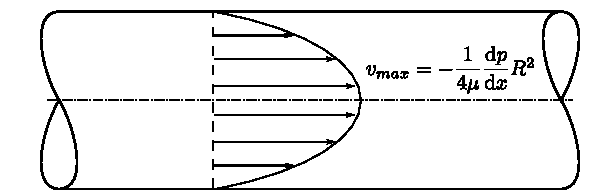
\includegraphics[width=\textwidth]{fig/inwendige_stroming/Laminair_snelheidsprofiel}
		}
	\end{frame}
%%%%%%%%%%%%%%%%%%%%%%%%%%%%%%%%%%%%%%%%%%%%%%%%%%%%%%%%%%%%%%%%%%%%%%%%%%%
  	\begin{frame}
		\frametitle{Gemiddelde snelheid}
		\only<1-2>{
			\begin{textblock}{5}(0,3)
            	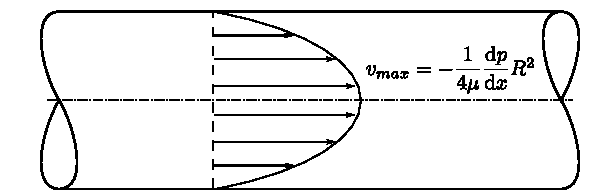
\includegraphics[width=5cm]{fig/inwendige_stroming/Laminair_snelheidsprofiel}
       		\end{textblock}
       		\vspace{2cm}
		}
		\only<1-2>{
			Debiet:
			\begin{equation*}
				\dot{V} = 2 \pi \int_0^R v_\mathrm{max} \left(1- \frac{r^2}{R^2}\right) r \diff r = v_\mathrm{max} \frac{\pi R^2}{2}
			\end{equation*}
		}
		\only<2-2>{
			Gemiddelde snelheid:
			\begin{equation}
				v_\mathrm{gem} = \frac{\dot{V}}{\pi R^2} = \frac{v_\mathrm{max}}{2} = - \frac{1}{8 \mu}\frac{\diff p}{\diff x} R^2
			\end{equation}
		}
	\end{frame}
%%%%%%%%%%%%%%%%%%%%%%%%%%%%%%%%%%%%%%%%%%%%%%%%%%%%%%%%%%%%%%%%%%%%%%%%%%%
  	\begin{frame}
		\frametitle{Drukval}
		\only<1-5>{
			\begin{equation*}
				v_\mathrm{gem} = - \frac{1}{8 \mu}\frac{\diff p}{\diff x} R^2
			\end{equation*}
		}
		\only<2-5>{
			\begin{equation*}
				\frac{\diff p}{\diff x} = - 8 \mu v_\mathrm{gem} \frac{1}{R^2}
			\end{equation*}
		}
		\only<3-5>{
			\hspace{5cm} $\Downarrow \quad  \begin{array}{rcl} \dfrac{\diff p}{\diff x} &=& -\dfrac{\Delta p}{L}\\ R &=& D/2 \end{array}$
		}
		\only<4-5>{
			\begin{equation*}
				\Delta p = 32 \mu v_\mathrm{gem} \frac{L}{D^2}
			\end{equation*}
		}
		\only<5-5>{
			\begin{equation*}
				\Delta p = \frac{1}{2} \rho v^2 \frac{64 \mu}{\rho v D} \frac{L}{D}
			\end{equation*}
		}
		\only<6-9>{
			\begin{equation*}
				\Delta p = \frac{1}{2} \rho v^2 \frac{64 \mu}{\rho v D} \frac{L}{D}
			\end{equation*}
		}
		\only<7-9>{
			\begin{equation*}
				\Delta p = \frac{1}{2} \rho v^2 \frac{64}{\mathrm{Re}} \frac{L}{D}
			\end{equation*}
		}
		\only<8-9>{
			\vspace{0.5cm}
			\begin{equation}
				\Delta p = \frac{1}{2} \rho v^2 f \frac{L}{D}
			\end{equation}
		}
		\only<9-9>{
			\vspace{0.5cm}
			\center
			wrijvingsfactor voor laminaire stroming $f = \dfrac{64}{\mathrm{Re}}$
		}
	\end{frame}
%%%%%%%%%%%%%%%%%%%%%%%%%%%%%%%%%%%%%%%%%%%%%%%%%%%%%%%%%%%%%%%%%%%%%%%%%%%
  	\section{Turbulente stroming}
  	\begin{frame}
		\frametitle{Empirische data}
		\center
		\only<1>{
			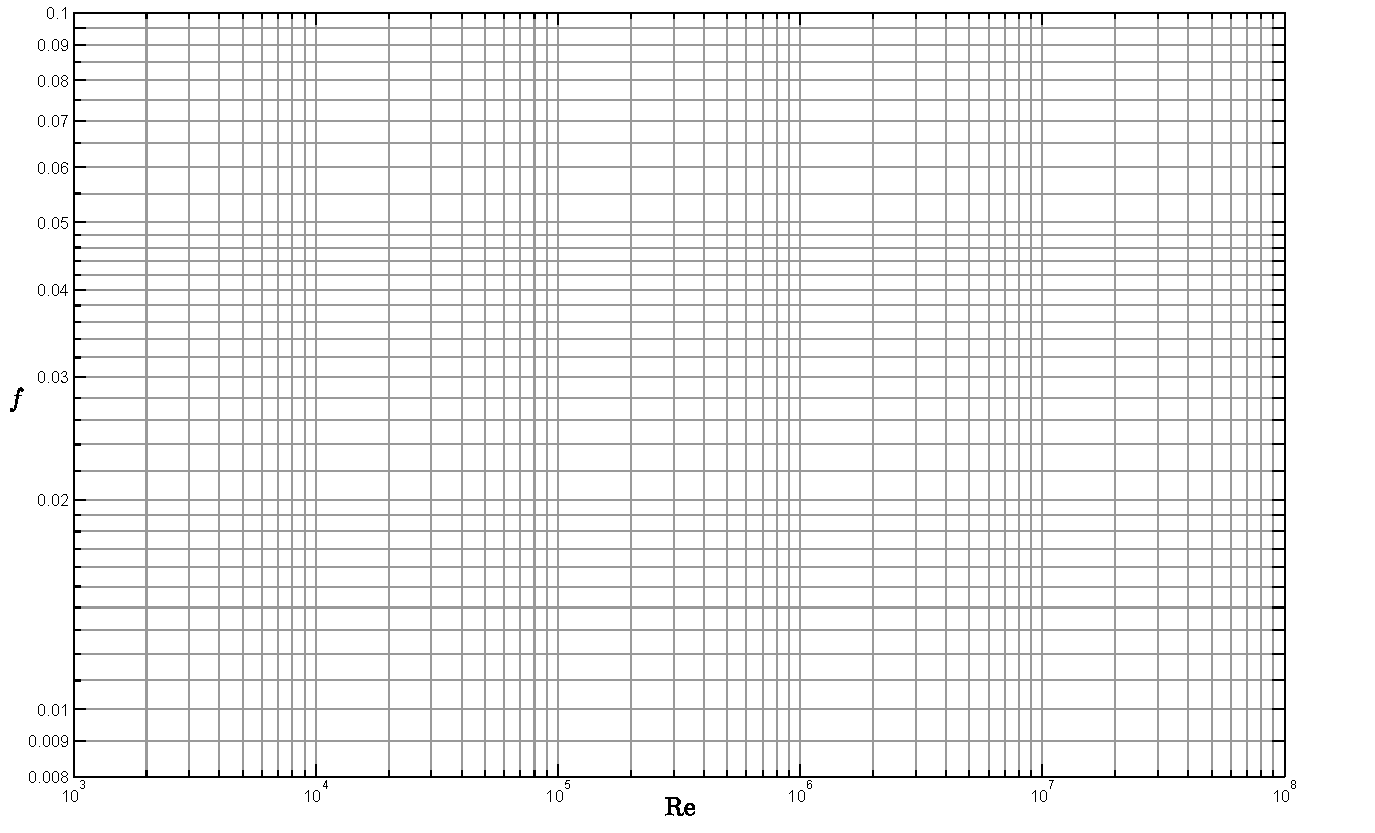
\includegraphics[width=\textwidth]{fig/stroming_in_leidingen/Moody_diagram_empirisch_leeg}
		}
		\only<2>{
			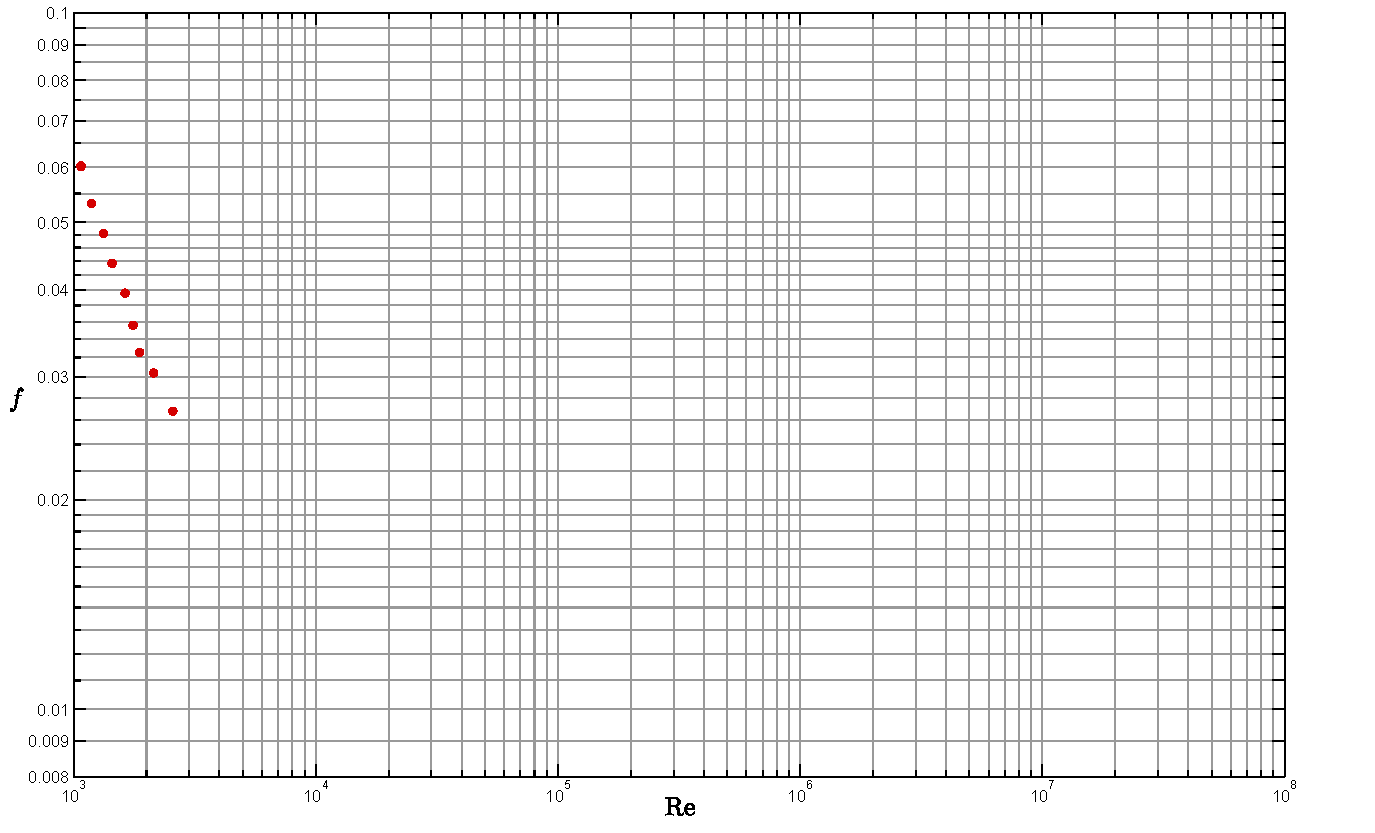
\includegraphics[width=\textwidth]{fig/stroming_in_leidingen/Moody_diagram_empirisch0_laminair}
		}
		\only<3>{
			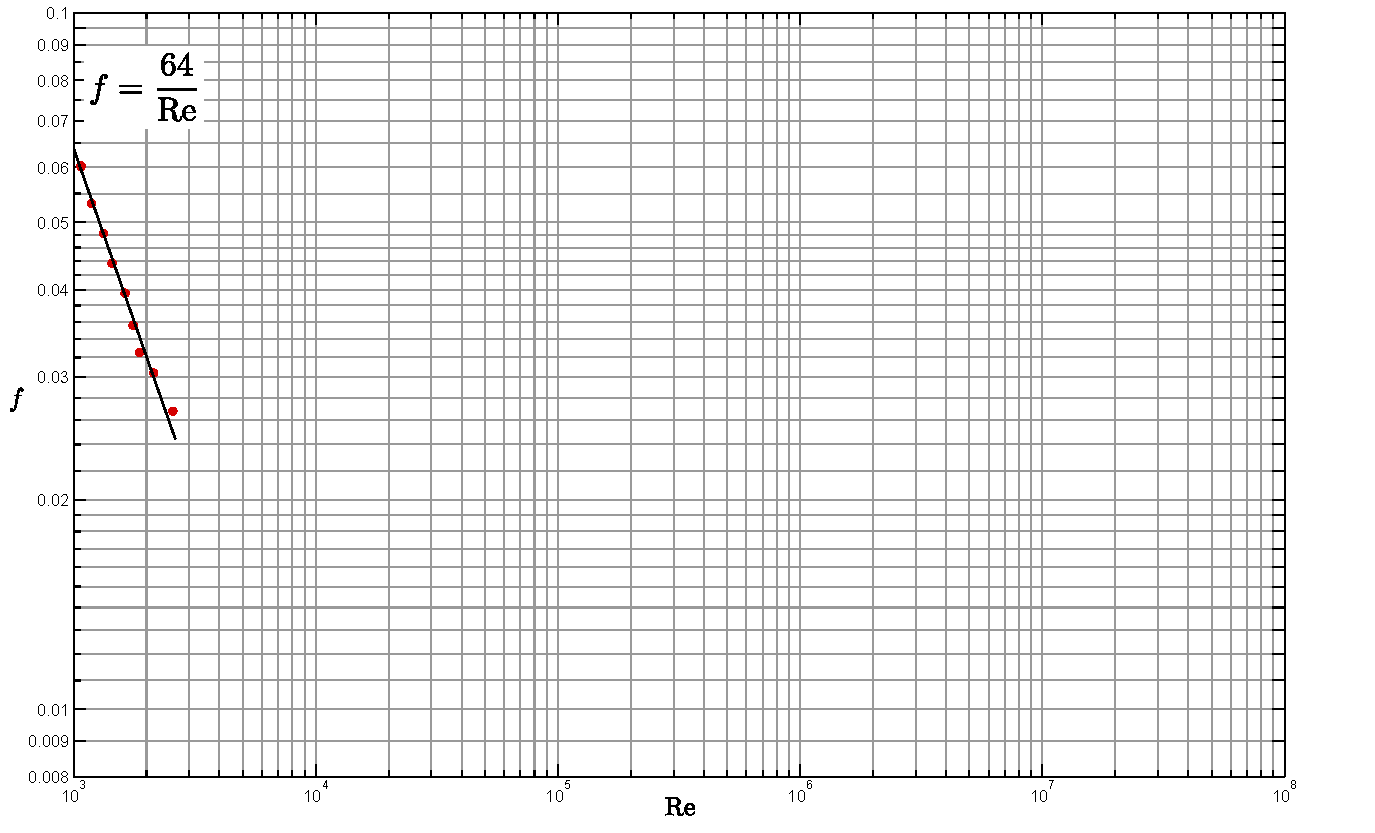
\includegraphics[width=\textwidth]{fig/stroming_in_leidingen/Moody_diagram_empirisch0_laminair_fit}
		}
		\only<4>{
			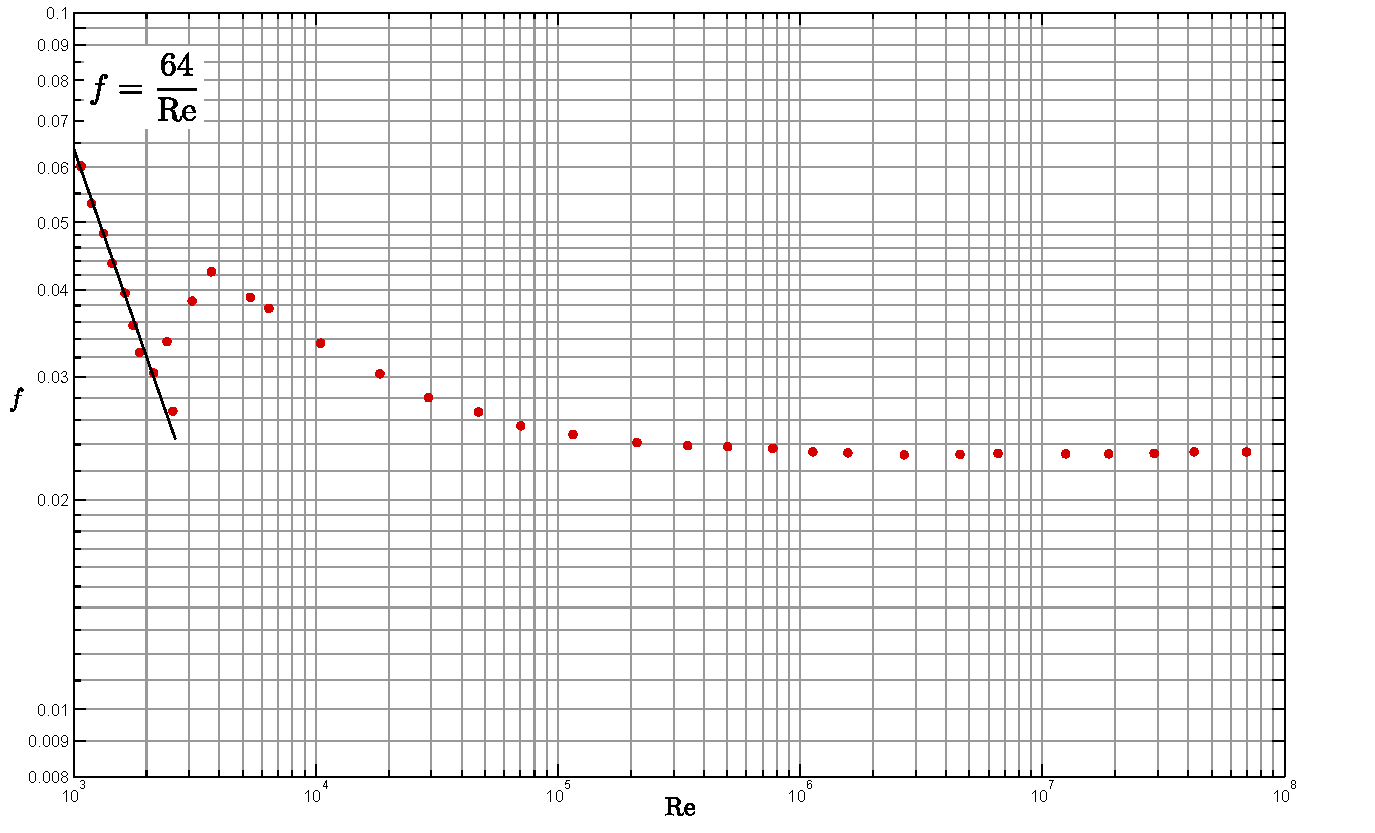
\includegraphics[width=\textwidth]{fig/stroming_in_leidingen/Moody_diagram_empirisch0}
		}
		\only<5>{
			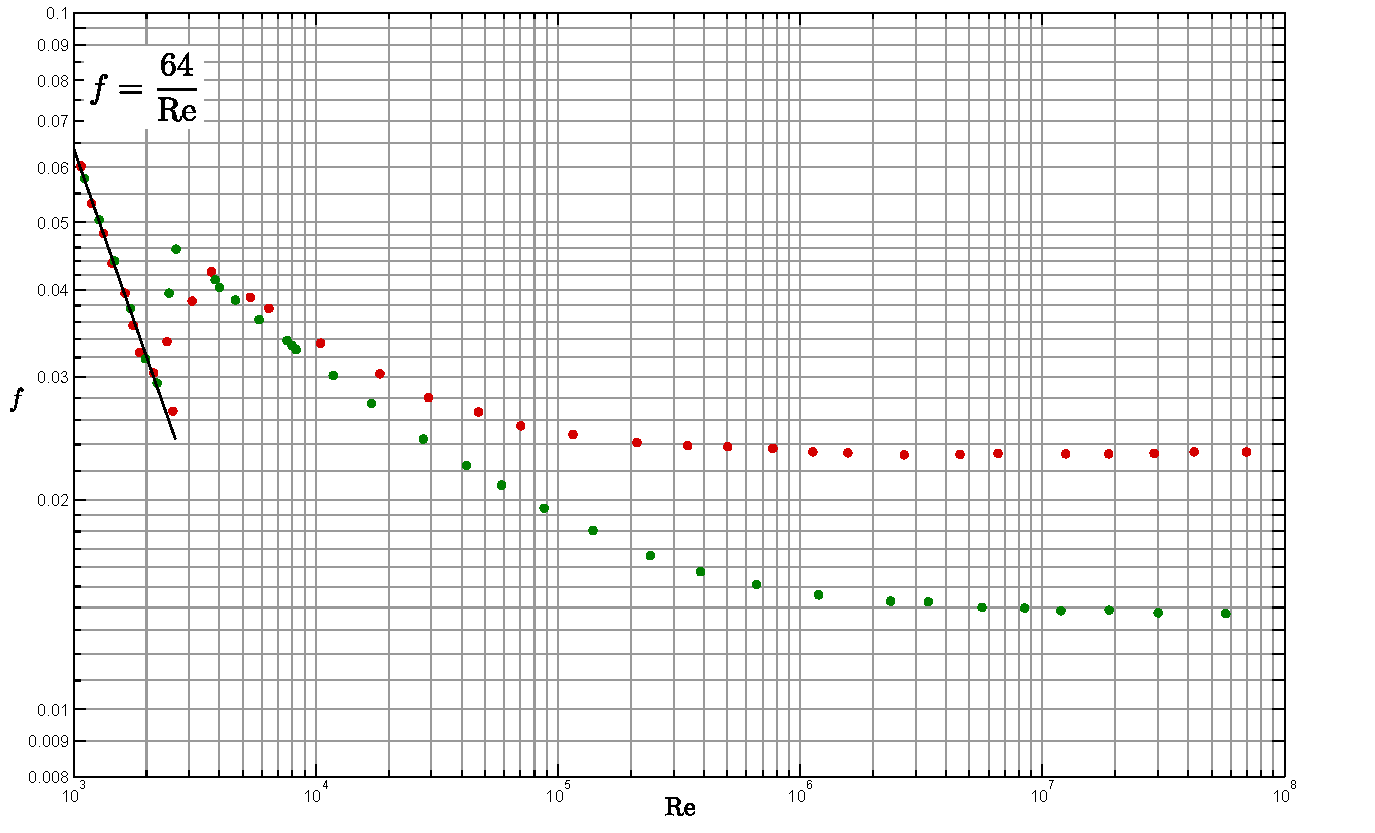
\includegraphics[width=\textwidth]{fig/stroming_in_leidingen/Moody_diagram_empirisch1}
		}
		\only<6>{
			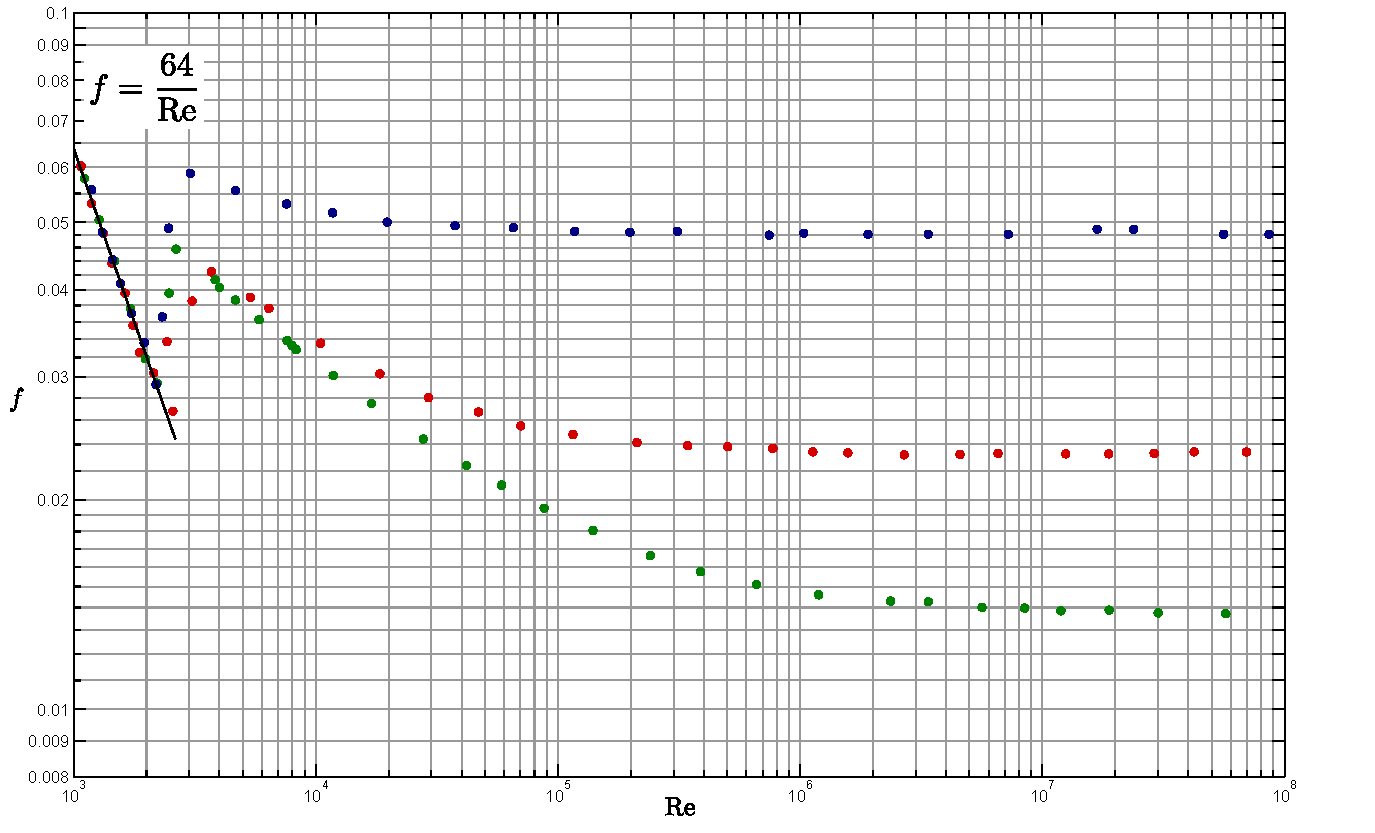
\includegraphics[width=\textwidth]{fig/stroming_in_leidingen/Moody_diagram_empirisch2}
		}
		\only<7>{
			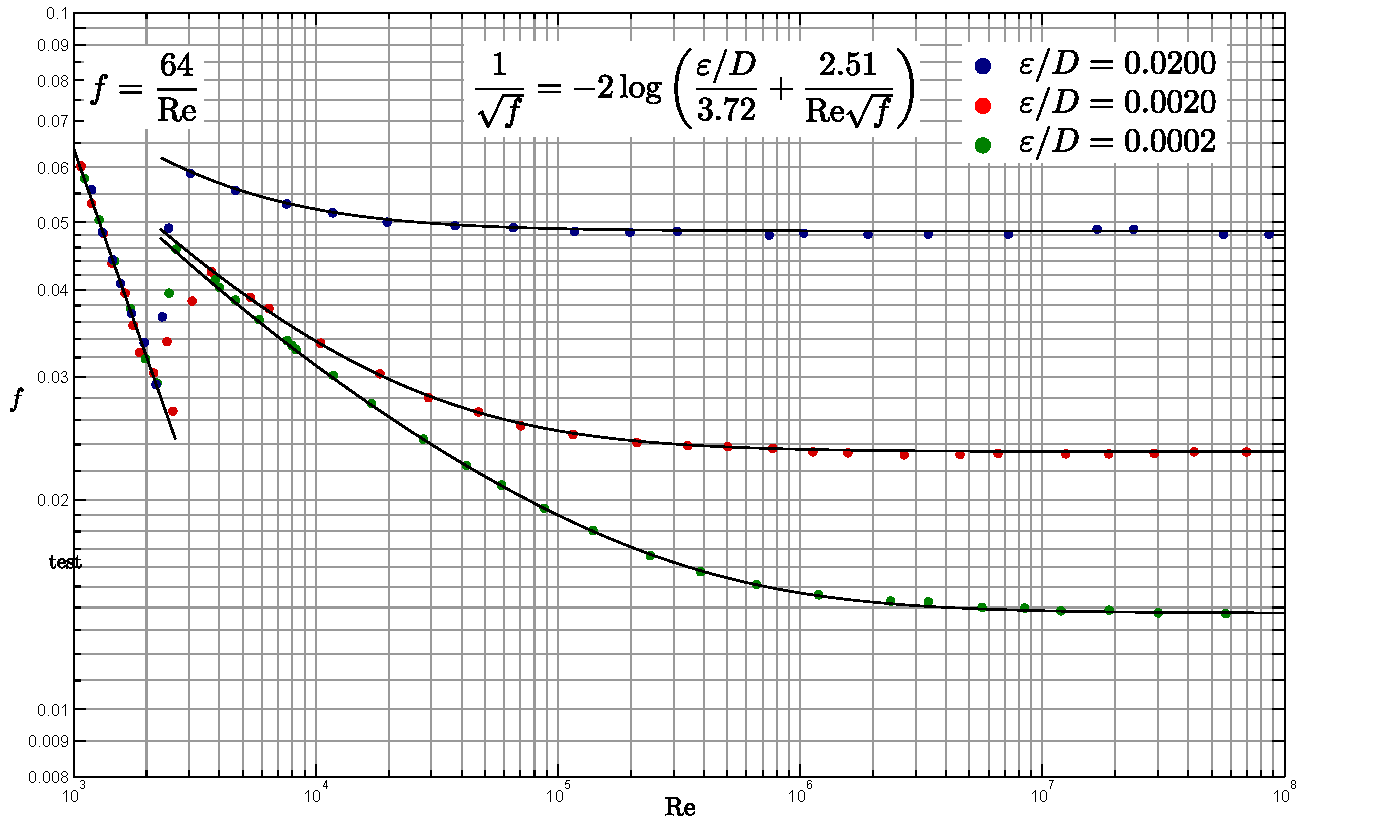
\includegraphics[width=\textwidth]{fig/stroming_in_leidingen/Moody_diagram_empirisch_turbulent_fit}
		}
		\only<8>{
			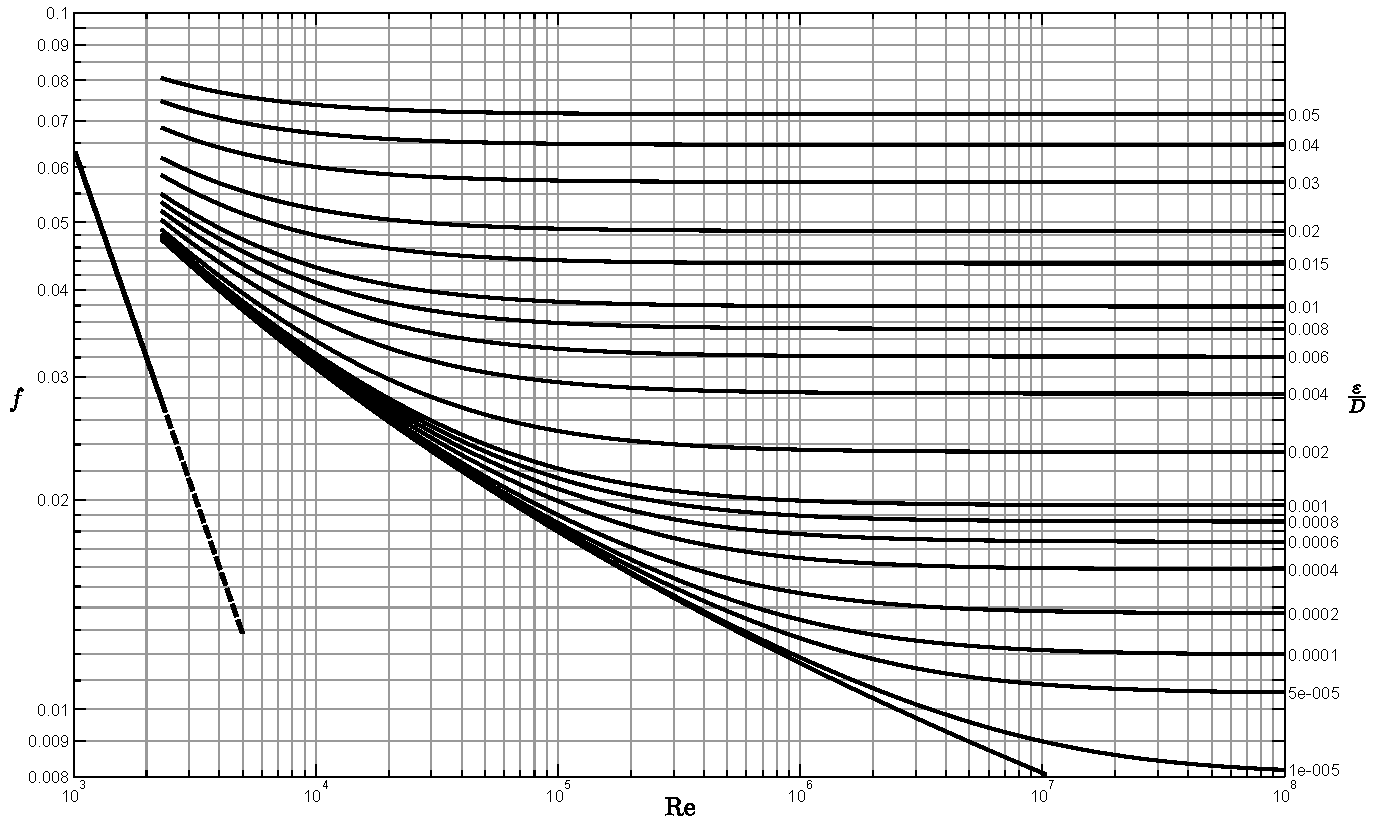
\includegraphics[width=\textwidth]{fig/stroming_in_leidingen/Moody_diagram}
		}
	\end{frame}
%%%%%%%%%%%%%%%%%%%%%%%%%%%%%%%%%%%%%%%%%%%%%%%%%%%%%%%%%%%%%%%%%%%%%%%%%%%
  	\begin{frame}
		\frametitle{Dimensieanalyse}
		\vspace{1cm}
		\begin{equation*}
			\Delta p = \phi(L,D,v,\mu,\rho,\varepsilon)
		\end{equation*}
		\vspace{0.5cm}
		\begin{equation*}
			\Delta p = f(Re,\varepsilon/D) \frac{1}{2}\rho v^2 \frac{L}{D}
		\end{equation*}
		\pause
		\center
		De wrijvingsfactor $f$ voor turbulente stroming moet bepaald worden met behulp van empirische data:
		
		Moody diagram
	\end{frame}
%%%%%%%%%%%%%%%%%%%%%%%%%%%%%%%%%%%%%%%%%%%%%%%%%%%%%%%%%%%%%%%%%%%%%%%%%%%
  	\begin{frame}
		\frametitle{Moody diagram}
		\center
		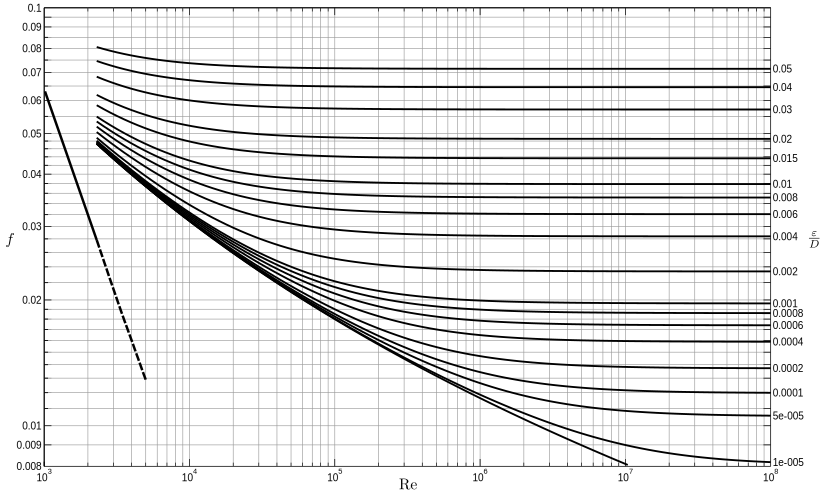
\includegraphics[width=\textwidth]{fig/stroming_in_leidingen/Moody_diagram_regimes}
	\end{frame}
%%%%%%%%%%%%%%%%%%%%%%%%%%%%%%%%%%%%%%%%%%%%%%%%%%%%%%%%%%%%%%%%%%%%%%%%%%%
  	\begin{frame}
		\frametitle{Gebruik van het Moody diagram}
		\center
		\only<1>{
			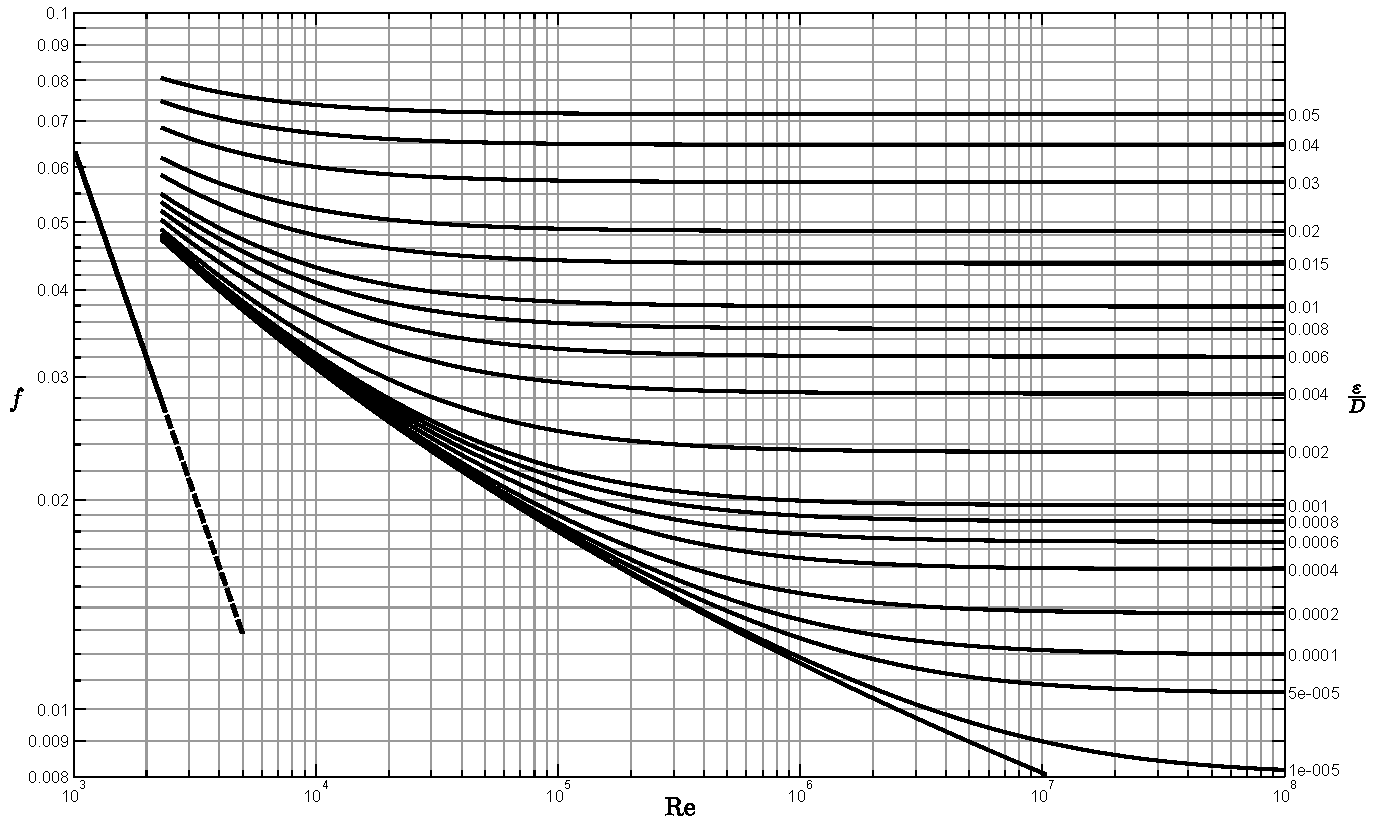
\includegraphics[width=\textwidth]{fig/stroming_in_leidingen/Moody_diagram_gebruik}
		}
		\only<2>{
			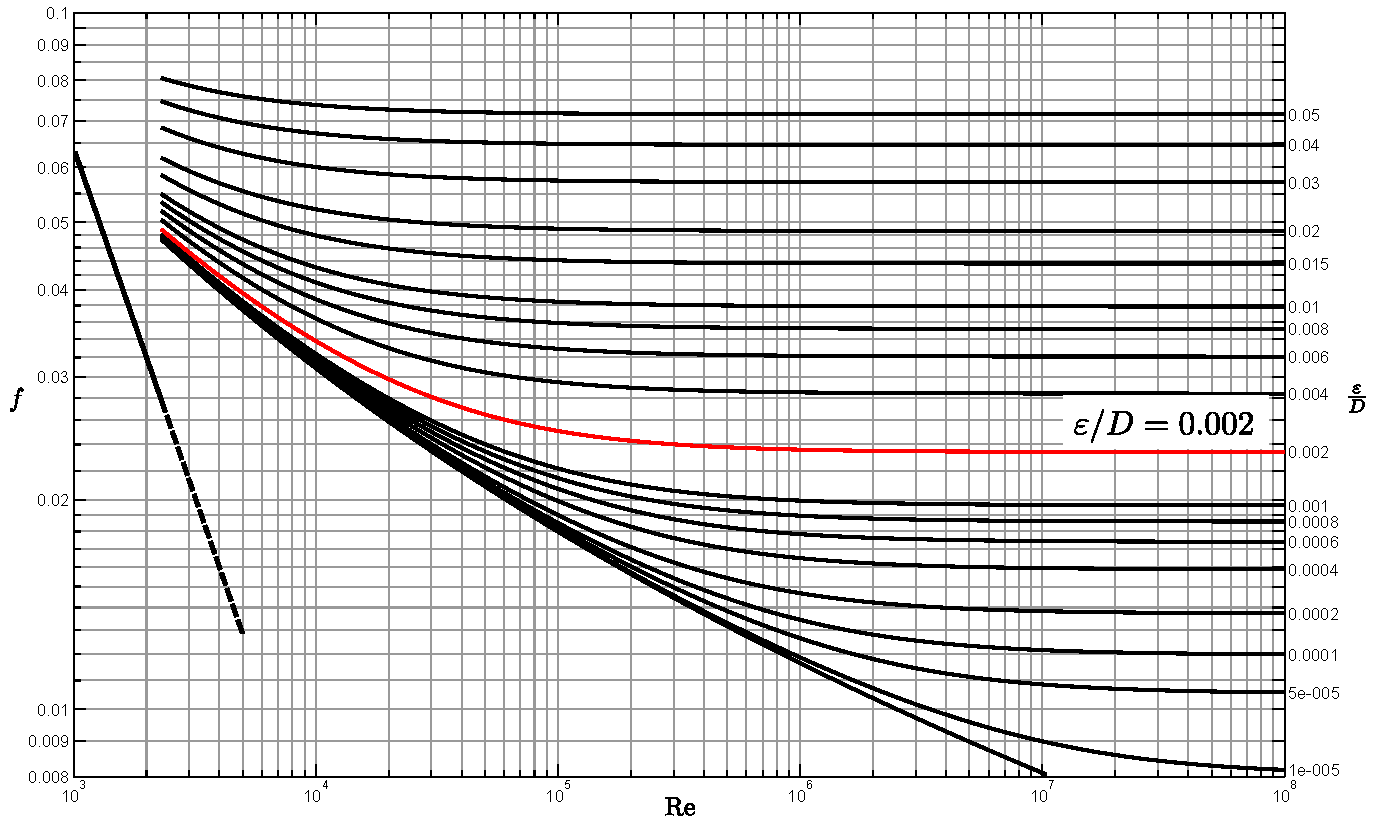
\includegraphics[width=\textwidth]{fig/stroming_in_leidingen/Moody_diagram_gebruik1}
		}
		\only<3>{
			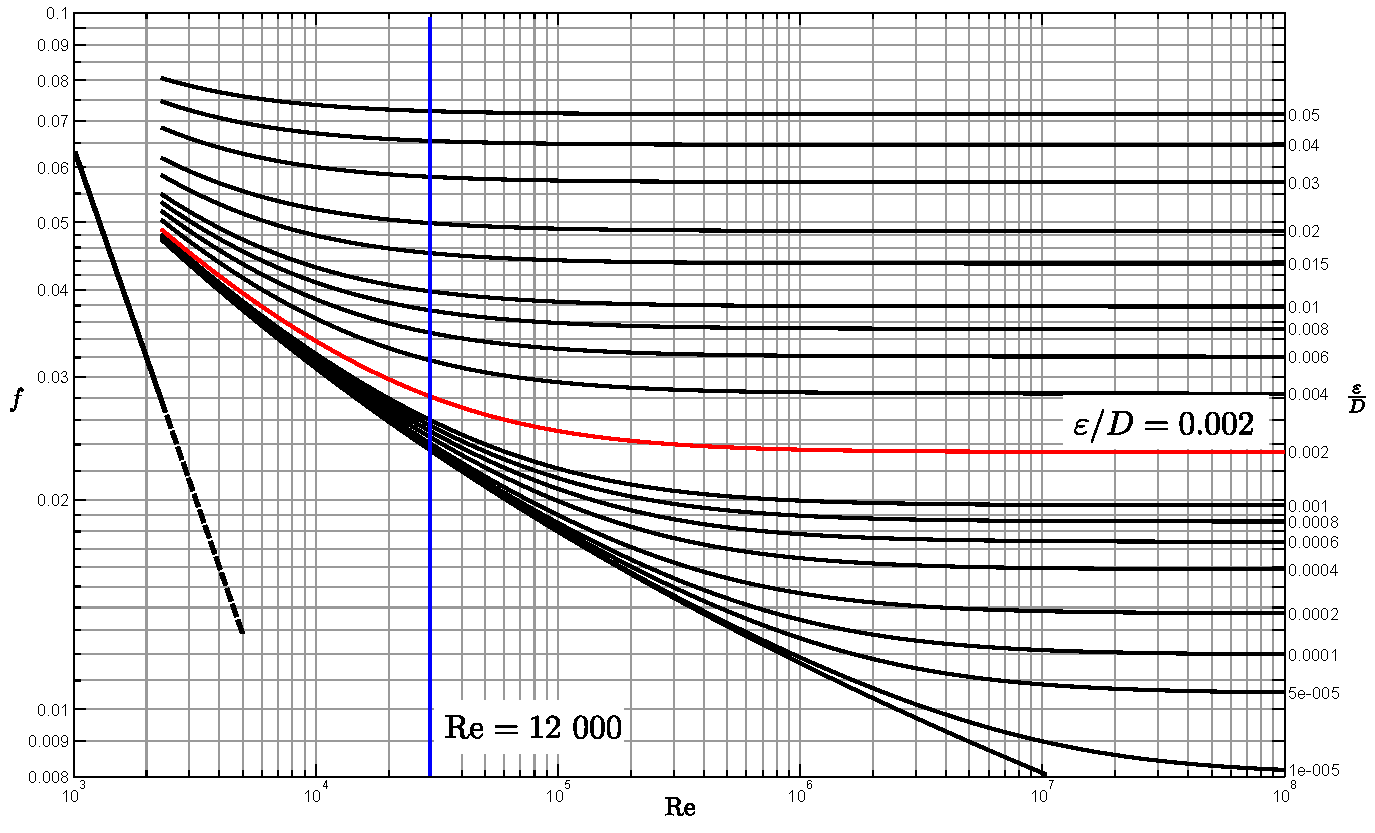
\includegraphics[width=\textwidth]{fig/stroming_in_leidingen/Moody_diagram_gebruik2}
		}
		\only<4>{
			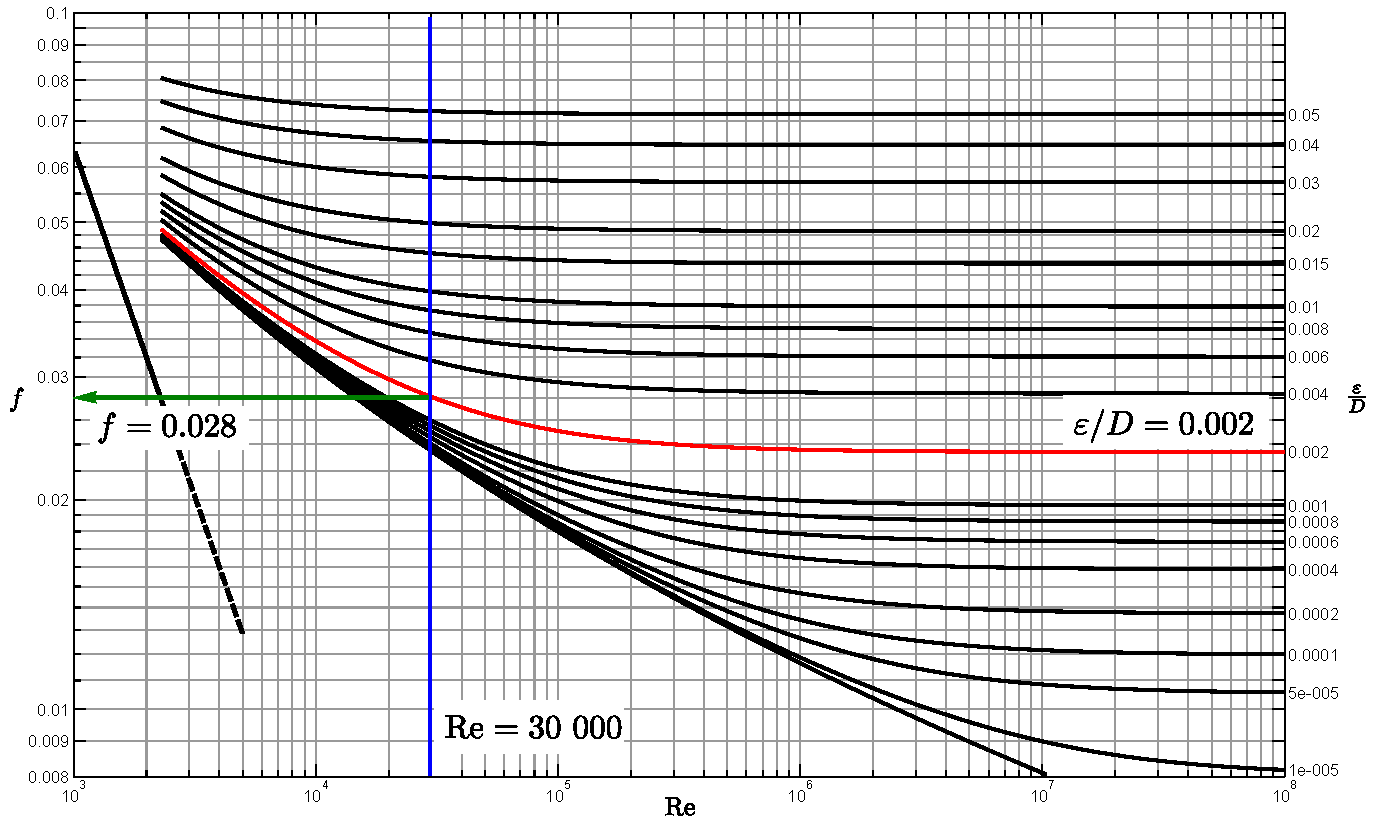
\includegraphics[width=\textwidth]{fig/stroming_in_leidingen/Moody_diagram_gebruik3}
		}
	\end{frame}
%%%%%%%%%%%%%%%%%%%%%%%%%%%%%%%%%%%%%%%%%%%%%%%%%%%%%%%%%%%%%%%%%%%%%%%%%%%
  	\begin{frame}
		\frametitle{Turbulent snelheidsprofiel}
		\vspace{0.5cm}
		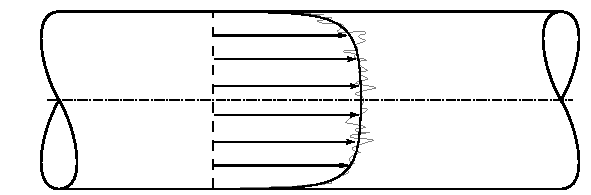
\includegraphics[width=\textwidth]{fig/inwendige_stroming/Turbulent_snelheidsprofiel}
		\pause
		\vspace{0.5cm}
		\begin{equation*}
			\frac{\bar{v}}{v_{\text{max}}} \approx \left(1- \frac{r}{R}\right)^{1/7}
		\end{equation*}
	\end{frame}
%%%%%%%%%%%%%%%%%%%%%%%%%%%%%%%%%%%%%%%%%%%%%%%%%%%%%%%%%%%%%%%%%%%%%%%%%%%
  	\begin{frame}
		\frametitle{Invloed van ruwheid}
		\vspace{1cm}
		\center
		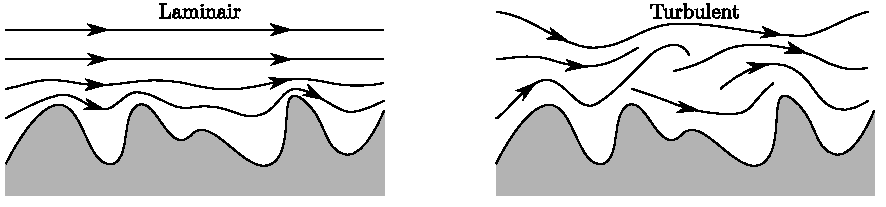
\includegraphics[width=\textwidth]{fig/stroming_in_leidingen/Ruwheid_laminair_turbulent}
		
		\pause
		\vspace{0.5cm}
		Bij laminaire stroming worden door de ruwheid geïnduceerde fluctuaties door de viskeuze krachten afgevlakt
		
		\pause
		\vspace{0.5cm}
		Bij turbulente stroming hebben door de ruwheid geïnduceerde fluctuaties invloed in de volledige stroming
	\end{frame}
%%%%%%%%%%%%%%%%%%%%%%%%%%%%%%%%%%%%%%%%%%%%%%%%%%%%%%%%%%%%%%%%%%%%%%%%%%%
\end{document}